\documentclass{standalone}
\usepackage{tikz}
\usetikzlibrary{patterns, positioning}


\begin{document}
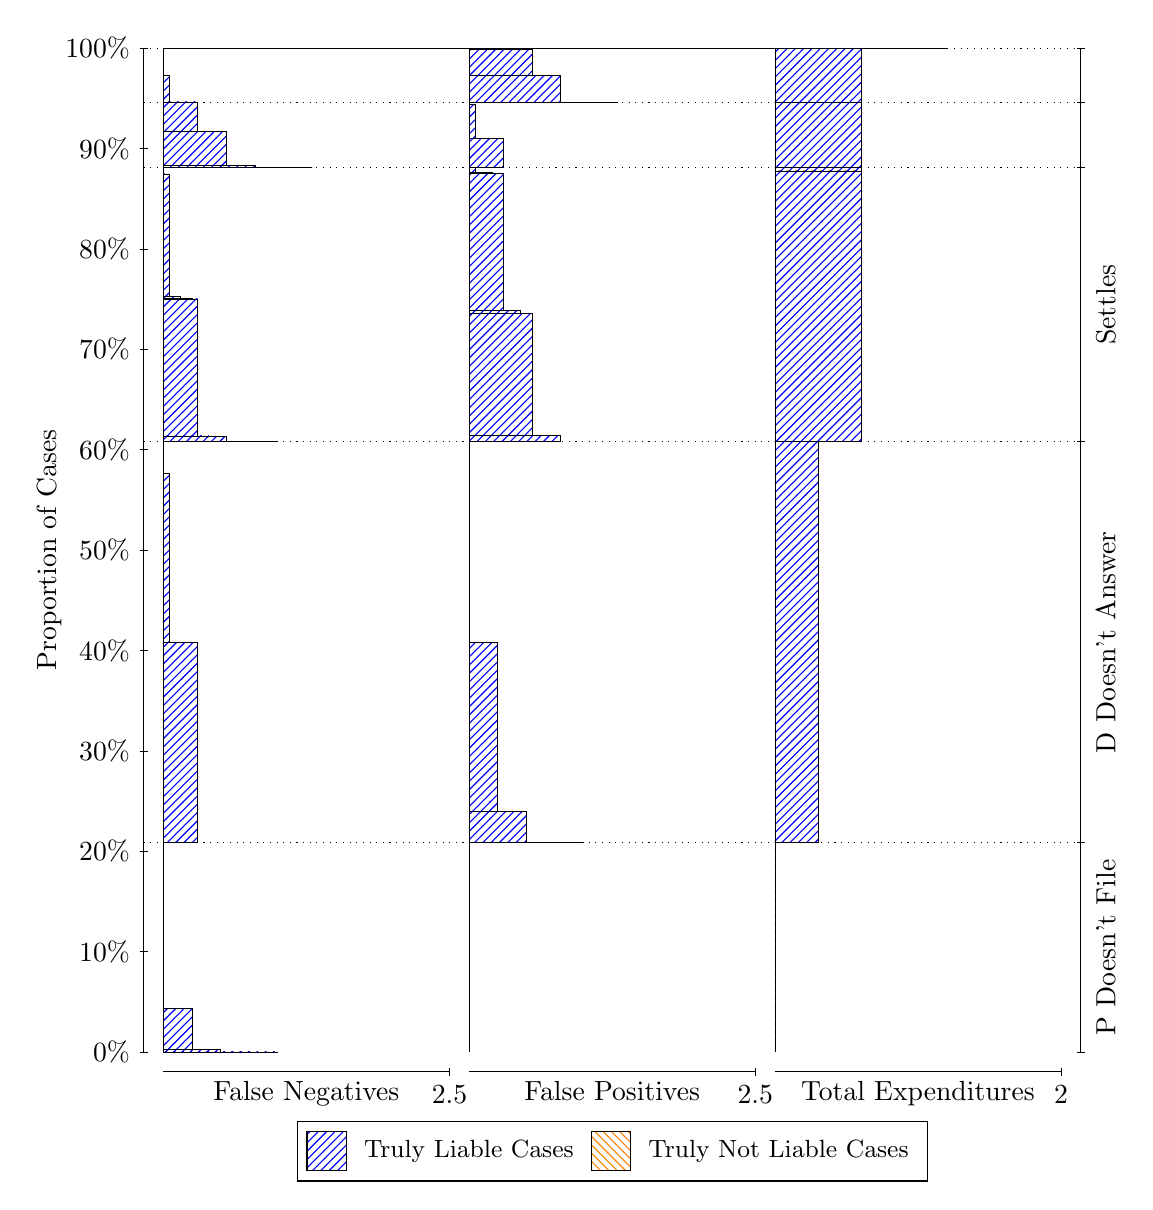
\begin{tikzpicture}
\draw[black, very thin] (1.5,1.75) -- (1.5,14.5);
\node[rotate=90, text=black, anchor=center] at (0.3, 8.125) {Proportion of Cases};
\draw[black, very thin] (1.45,1.75) -- (1.55,1.75);
\node[text=black, anchor=east] at (1.45, 1.75) {0\%};
\draw[black, very thin] (1.45,3.025) -- (1.55,3.025);
\node[text=black, anchor=east] at (1.45, 3.025) {10\%};
\draw[black, very thin] (1.45,4.3) -- (1.55,4.3);
\node[text=black, anchor=east] at (1.45, 4.3) {20\%};
\draw[black, very thin] (1.45,5.575) -- (1.55,5.575);
\node[text=black, anchor=east] at (1.45, 5.575) {30\%};
\draw[black, very thin] (1.45,6.85) -- (1.55,6.85);
\node[text=black, anchor=east] at (1.45, 6.85) {40\%};
\draw[black, very thin] (1.45,8.125) -- (1.55,8.125);
\node[text=black, anchor=east] at (1.45, 8.125) {50\%};
\draw[black, very thin] (1.45,9.4) -- (1.55,9.4);
\node[text=black, anchor=east] at (1.45, 9.4) {60\%};
\draw[black, very thin] (1.45,10.675) -- (1.55,10.675);
\node[text=black, anchor=east] at (1.45, 10.675) {70\%};
\draw[black, very thin] (1.45,11.95) -- (1.55,11.95);
\node[text=black, anchor=east] at (1.45, 11.95) {80\%};
\draw[black, very thin] (1.45,13.225) -- (1.55,13.225);
\node[text=black, anchor=east] at (1.45, 13.225) {90\%};
\draw[black, very thin] (1.45,14.5) -- (1.55,14.5);
\node[text=black, anchor=east] at (1.45, 14.5) {100\%};

\draw[black, very thin] (13.4,1.75) -- (13.4,14.5);
\draw[black, very thin] (13.35,1.75) -- (13.45,1.75);
\node[anchor=west] at (13.35, 1.75) {};
\draw[black, very thin] (13.35,4.4079) -- (13.45,4.4079);
\node[anchor=west] at (13.35, 4.4079) {};
\draw[black, very thin] (13.35,9.5007) -- (13.45,9.5007);
\node[anchor=west] at (13.35, 9.5007) {};
\draw[black, very thin] (13.35,12.981) -- (13.45,12.981);
\node[anchor=west] at (13.35, 12.981) {};
\draw[black, very thin] (13.35,13.811) -- (13.45,13.811);
\node[anchor=west] at (13.35, 13.811) {};
\draw[black, very thin] (13.35,14.493) -- (13.45,14.493);
\node[anchor=west] at (13.35, 14.493) {};
\draw[black, very thin] (13.35,14.5) -- (13.45,14.5);
\node[anchor=west] at (13.35, 14.5) {};

\draw[black, very thin, pattern color=blue, pattern=north east lines] (1.75,1.75) rectangle (3.2033,1.75);
\draw[black, very thin, pattern color=blue, pattern=north east lines] (1.75,1.75) rectangle (2.84,1.7502);
\draw[black, very thin, pattern color=blue, pattern=north east lines] (1.75,1.7502) rectangle (2.4767,1.7818);
\draw[black, very thin, pattern color=blue, pattern=north east lines] (1.75,1.7818) rectangle (2.1133,2.3054);
\draw[black, very thin, pattern color=orange, pattern=north west lines] (1.75,2.3054) rectangle (1.75,2.3054);
\draw[black, very thin, pattern color=blue, pattern=north east lines] (1.75,2.3054) rectangle (1.75,4.4079);
\draw[black, very thin, pattern color=blue, pattern=north east lines] (1.75,4.4079) rectangle (2.186,6.9537);
\draw[black, very thin, pattern color=blue, pattern=north east lines] (1.75,6.9537) rectangle (1.8227,9.0984);
\draw[black, very thin, pattern color=orange, pattern=north west lines] (1.75,9.0984) rectangle (1.75,9.0984);
\draw[black, very thin, pattern color=blue, pattern=north east lines] (1.75,9.0984) rectangle (1.75,9.5007);
\draw[black, very thin, pattern color=blue, pattern=north east lines] (1.75,9.5007) rectangle (3.2033,9.5007);
\draw[black, very thin, pattern color=blue, pattern=north east lines] (1.75,9.5007) rectangle (3.058,9.5007);
\draw[black, very thin, pattern color=blue, pattern=north east lines] (1.75,9.5007) rectangle (2.9127,9.5007);
\draw[black, very thin, pattern color=blue, pattern=north east lines] (1.75,9.5007) rectangle (2.84,9.5007);
\draw[black, very thin, pattern color=blue, pattern=north east lines] (1.75,9.5007) rectangle (2.6947,9.5007);
\draw[black, very thin, pattern color=blue, pattern=north east lines] (1.75,9.5007) rectangle (2.5493,9.565);
\draw[black, very thin, pattern color=blue, pattern=north east lines] (1.75,9.565) rectangle (2.4767,9.5651);
\draw[black, very thin, pattern color=blue, pattern=north east lines] (1.75,9.5651) rectangle (2.3313,9.5731);
\draw[black, very thin, pattern color=blue, pattern=north east lines] (1.75,9.5731) rectangle (2.186,11.313);
\draw[black, very thin, pattern color=blue, pattern=north east lines] (1.75,11.313) rectangle (2.1133,11.317);
\draw[black, very thin, pattern color=blue, pattern=north east lines] (1.75,11.317) rectangle (1.968,11.35);
\draw[black, very thin, pattern color=blue, pattern=north east lines] (1.75,11.35) rectangle (1.8227,12.901);
\draw[black, very thin, pattern color=orange, pattern=north west lines] (1.75,12.901) rectangle (1.75,12.901);
\draw[black, very thin, pattern color=blue, pattern=north east lines] (1.75,12.901) rectangle (1.75,12.981);
\draw[black, very thin, pattern color=blue, pattern=north east lines] (1.75,12.981) rectangle (3.6393,12.981);
\draw[black, very thin, pattern color=blue, pattern=north east lines] (1.75,12.981) rectangle (3.276,12.981);
\draw[black, very thin, pattern color=blue, pattern=north east lines] (1.75,12.981) rectangle (2.9127,13.012);
\draw[black, very thin, pattern color=blue, pattern=north east lines] (1.75,13.012) rectangle (2.5493,13.444);
\draw[black, very thin, pattern color=blue, pattern=north east lines] (1.75,13.444) rectangle (2.186,13.811);
\draw[black, very thin, pattern color=orange, pattern=north west lines] (1.75,13.811) rectangle (1.75,13.811);
\draw[black, very thin, pattern color=blue, pattern=north east lines] (1.75,13.811) rectangle (2.186,13.815);
\draw[black, very thin, pattern color=blue, pattern=north east lines] (1.75,13.815) rectangle (1.8227,14.156);
\draw[black, very thin, pattern color=orange, pattern=north west lines] (1.75,14.156) rectangle (1.75,14.156);
\draw[black, very thin, pattern color=blue, pattern=north east lines] (1.75,14.156) rectangle (1.75,14.493);
\draw[black, very thin, pattern color=blue, pattern=north east lines] (1.75,14.493) rectangle (5.8193,14.493);
\draw[black, very thin, pattern color=blue, pattern=north east lines] (1.75,14.493) rectangle (5.456,14.493);
\draw[black, very thin, pattern color=blue, pattern=north east lines] (1.75,14.493) rectangle (5.0927,14.493);
\draw[black, very thin, pattern color=blue, pattern=north east lines] (1.75,14.493) rectangle (4.7293,14.495);
\draw[black, very thin, pattern color=blue, pattern=north east lines] (1.75,14.495) rectangle (4.366,14.495);
\draw[black, very thin, pattern color=blue, pattern=north east lines] (1.75,14.495) rectangle (4.0027,14.495);
\draw[black, very thin, pattern color=blue, pattern=north east lines] (1.75,14.495) rectangle (1.968,14.495);
\draw[black, very thin, pattern color=orange, pattern=north west lines] (1.75,14.495) rectangle (1.75,14.495);
\draw[black, very thin, pattern color=blue, pattern=north east lines] (1.75,14.495) rectangle (1.75,14.5);
\draw[black, very thin, pattern color=orange, pattern=north west lines] (5.6333,1.75) rectangle (5.6333,1.75);
\draw[black, very thin, pattern color=blue, pattern=north east lines] (5.6333,1.75) rectangle (5.6333,4.4079);
\draw[black, very thin, pattern color=orange, pattern=north west lines] (5.6333,4.4079) rectangle (7.0867,4.4079);
\draw[black, very thin, pattern color=blue, pattern=north east lines] (5.6333,4.4079) rectangle (7.0867,4.4079);
\draw[black, very thin, pattern color=blue, pattern=north east lines] (5.6333,4.4079) rectangle (6.7233,4.4106);
\draw[black, very thin, pattern color=blue, pattern=north east lines] (5.6333,4.4106) rectangle (6.36,4.8102);
\draw[black, very thin, pattern color=blue, pattern=north east lines] (5.6333,4.8102) rectangle (5.9967,6.9549);
\draw[black, very thin, pattern color=blue, pattern=north east lines] (5.6333,6.9549) rectangle (5.6333,9.5007);
\draw[black, very thin, pattern color=orange, pattern=north west lines] (5.6333,9.5007) rectangle (6.796,9.5007);
\draw[black, very thin, pattern color=blue, pattern=north east lines] (5.6333,9.5007) rectangle (6.796,9.576);
\draw[black, very thin, pattern color=orange, pattern=north west lines] (5.6333,9.576) rectangle (6.6507,9.576);
\draw[black, very thin, pattern color=blue, pattern=north east lines] (5.6333,9.576) rectangle (6.6507,9.578);
\draw[black, very thin, pattern color=orange, pattern=north west lines] (5.6333,9.578) rectangle (6.5053,9.578);
\draw[black, very thin, pattern color=blue, pattern=north east lines] (5.6333,9.578) rectangle (6.5053,9.5811);
\draw[black, very thin, pattern color=blue, pattern=north east lines] (5.6333,9.5811) rectangle (6.4327,11.132);
\draw[black, very thin, pattern color=blue, pattern=north east lines] (5.6333,11.132) rectangle (6.2873,11.165);
\draw[black, very thin, pattern color=blue, pattern=north east lines] (5.6333,11.165) rectangle (6.142,11.169);
\draw[black, very thin, pattern color=blue, pattern=north east lines] (5.6333,11.169) rectangle (6.0693,12.909);
\draw[black, very thin, pattern color=blue, pattern=north east lines] (5.6333,12.909) rectangle (5.924,12.917);
\draw[black, very thin, pattern color=blue, pattern=north east lines] (5.6333,12.917) rectangle (5.7787,12.917);
\draw[black, very thin, pattern color=blue, pattern=north east lines] (5.6333,12.917) rectangle (5.706,12.981);
\draw[black, very thin, pattern color=blue, pattern=north east lines] (5.6333,12.981) rectangle (5.6333,12.981);
\draw[black, very thin, pattern color=orange, pattern=north west lines] (5.6333,12.981) rectangle (6.0693,12.981);
\draw[black, very thin, pattern color=blue, pattern=north east lines] (5.6333,12.981) rectangle (6.0693,13.348);
\draw[black, very thin, pattern color=blue, pattern=north east lines] (5.6333,13.348) rectangle (5.706,13.78);
\draw[black, very thin, pattern color=blue, pattern=north east lines] (5.6333,13.78) rectangle (5.6333,13.811);
\draw[black, very thin, pattern color=orange, pattern=north west lines] (5.6333,13.811) rectangle (7.5227,13.811);
\draw[black, very thin, pattern color=blue, pattern=north east lines] (5.6333,13.811) rectangle (7.5227,13.811);
\draw[black, very thin, pattern color=blue, pattern=north east lines] (5.6333,13.811) rectangle (7.1593,13.814);
\draw[black, very thin, pattern color=blue, pattern=north east lines] (5.6333,13.814) rectangle (6.796,14.148);
\draw[black, very thin, pattern color=blue, pattern=north east lines] (5.6333,14.148) rectangle (6.4327,14.489);
\draw[black, very thin, pattern color=blue, pattern=north east lines] (5.6333,14.489) rectangle (6.0693,14.493);
\draw[black, very thin, pattern color=orange, pattern=north west lines] (5.6333,14.493) rectangle (9.7027,14.493);
\draw[black, very thin, pattern color=blue, pattern=north east lines] (5.6333,14.493) rectangle (9.7027,14.493);
\draw[black, very thin, pattern color=orange, pattern=north west lines] (5.6333,14.493) rectangle (9.3393,14.493);
\draw[black, very thin, pattern color=blue, pattern=north east lines] (5.6333,14.493) rectangle (9.3393,14.493);
\draw[black, very thin, pattern color=orange, pattern=north west lines] (5.6333,14.493) rectangle (8.976,14.493);
\draw[black, very thin, pattern color=blue, pattern=north east lines] (5.6333,14.493) rectangle (8.976,14.493);
\draw[black, very thin, pattern color=orange, pattern=north west lines] (5.6333,14.493) rectangle (8.6127,14.493);
\draw[black, very thin, pattern color=blue, pattern=north east lines] (5.6333,14.493) rectangle (8.6127,14.495);
\draw[black, very thin, pattern color=blue, pattern=north east lines] (5.6333,14.495) rectangle (8.2493,14.498);
\draw[black, very thin, pattern color=blue, pattern=north east lines] (5.6333,14.498) rectangle (7.886,14.498);
\draw[black, very thin, pattern color=blue, pattern=north east lines] (5.6333,14.498) rectangle (7.5227,14.498);
\draw[black, very thin, pattern color=blue, pattern=north east lines] (5.6333,14.498) rectangle (7.1593,14.498);
\draw[black, very thin, pattern color=orange, pattern=north west lines] (5.6333,14.498) rectangle (5.6333,14.498);
\draw[black, very thin, pattern color=blue, pattern=north east lines] (5.6333,14.498) rectangle (5.6333,14.5);
\draw[black, very thin, pattern color=orange, pattern=north west lines] (9.5167,1.75) rectangle (9.5167,1.75);
\draw[black, very thin, pattern color=blue, pattern=north east lines] (9.5167,1.75) rectangle (9.5167,4.4079);
\draw[black, very thin, pattern color=orange, pattern=north west lines] (9.5167,4.4079) rectangle (10.062,4.4079);
\draw[black, very thin, pattern color=blue, pattern=north east lines] (9.5167,4.4079) rectangle (10.062,9.5007);
\draw[black, very thin, pattern color=orange, pattern=north west lines] (9.5167,9.5007) rectangle (10.607,9.5007);
\draw[black, very thin, pattern color=blue, pattern=north east lines] (9.5167,9.5007) rectangle (10.607,12.931);
\draw[black, very thin, pattern color=orange, pattern=north west lines] (9.5167,12.931) rectangle (10.607,12.931);
\draw[black, very thin, pattern color=blue, pattern=north east lines] (9.5167,12.931) rectangle (10.607,12.939);
\draw[black, very thin, pattern color=orange, pattern=north west lines] (9.5167,12.939) rectangle (10.607,12.939);
\draw[black, very thin, pattern color=blue, pattern=north east lines] (9.5167,12.939) rectangle (10.607,12.981);
\draw[black, very thin, pattern color=orange, pattern=north west lines] (9.5167,12.981) rectangle (10.607,12.981);
\draw[black, very thin, pattern color=blue, pattern=north east lines] (9.5167,12.981) rectangle (10.607,13.811);
\draw[black, very thin, pattern color=orange, pattern=north west lines] (9.5167,13.811) rectangle (10.607,13.811);
\draw[black, very thin, pattern color=blue, pattern=north east lines] (9.5167,13.811) rectangle (10.607,14.493);
\draw[black, very thin, pattern color=orange, pattern=north west lines] (9.5167,14.493) rectangle (11.697,14.493);
\draw[black, very thin, pattern color=blue, pattern=north east lines] (9.5167,14.493) rectangle (11.697,14.5);
\draw[black, dotted] (1.5,4.4079) -- (13.4,4.4079);
\draw[black, dotted] (1.5,9.5007) -- (13.4,9.5007);
\draw[black, dotted] (1.5,12.981) -- (13.4,12.981);
\draw[black, dotted] (1.5,13.811) -- (13.4,13.811);
\draw[black, dotted] (1.5,14.493) -- (13.4,14.493);
\draw[black, very thin] (1.75,1.5) -- (5.3833,1.5);
\node[text=black, anchor=north] at (3.5667, 1.5) {False Negatives};
\draw[black, very thin] (5.3833,1.45) -- (5.3833,1.55);
\node[text=black, anchor=north] at (5.3833, 1.45) {2.5};

\draw[black, very thin] (5.6333,1.5) -- (9.2667,1.5);
\node[text=black, anchor=north] at (7.45, 1.5) {False Positives};
\draw[black, very thin] (9.2667,1.45) -- (9.2667,1.55);
\node[text=black, anchor=north] at (9.2667, 1.45) {2.5};

\draw[black, very thin] (9.5167,1.5) -- (13.15,1.5);
\node[text=black, anchor=north] at (11.333, 1.5) {Total Expenditures};
\draw[black, very thin] (13.15,1.45) -- (13.15,1.55);
\node[text=black, anchor=north] at (13.15, 1.45) {2};

\node[text=black, centered, rotate=90] at (13.72, 3.0789) {P Doesn't File};
\node[text=black, centered, rotate=90] at (13.72, 6.9543) {D Doesn't Answer};
\node[text=black, centered, rotate=90] at (13.72, 11.241) {Settles};




\draw (7.449999999999999,1.5) node[draw=none] (baseCoordinate) {};
\begin{scope}[align=center]
        \matrix[scale=0.5, draw=black, below=0.5cm of baseCoordinate, nodes={draw}, column sep=0.1cm]{
            \node[rectangle, draw, minimum width=0.5cm, minimum height=0.5cm, pattern color=blue, pattern=north east lines] {}; &
            \node[draw=none, font=\small, text=black] (B) {Truly Liable Cases}; &
            \node[rectangle, draw, minimum width=0.5cm, minimum height=0.5cm, pattern color=orange, pattern=north west lines] {}; &
            \node[draw=none, font=\small, text=black] (B) {Truly Not Liable Cases}; \\
            };
\end{scope}

\end{tikzpicture}
\end{document}